\documentclass{ximera}

\graphicspath{{./graphics/}}

\title{Quadric Surfaces}
\begin{document}
\begin{abstract}
\end{abstract}
\maketitle


In this activity, we introduce and classify quadric surfaces, which form an important family of surfaces.

\section{Definition of a Quadric Surface}

You might remember studying conic sections, such as parabolas, circles, ellipses, and hyperbolas. These are curves in the plane that arise through polynomial equations of degree two in two variables.

\begin{image}
\begin{tikzpicture}
\node[inner sep=0pt] at (0,0)
    {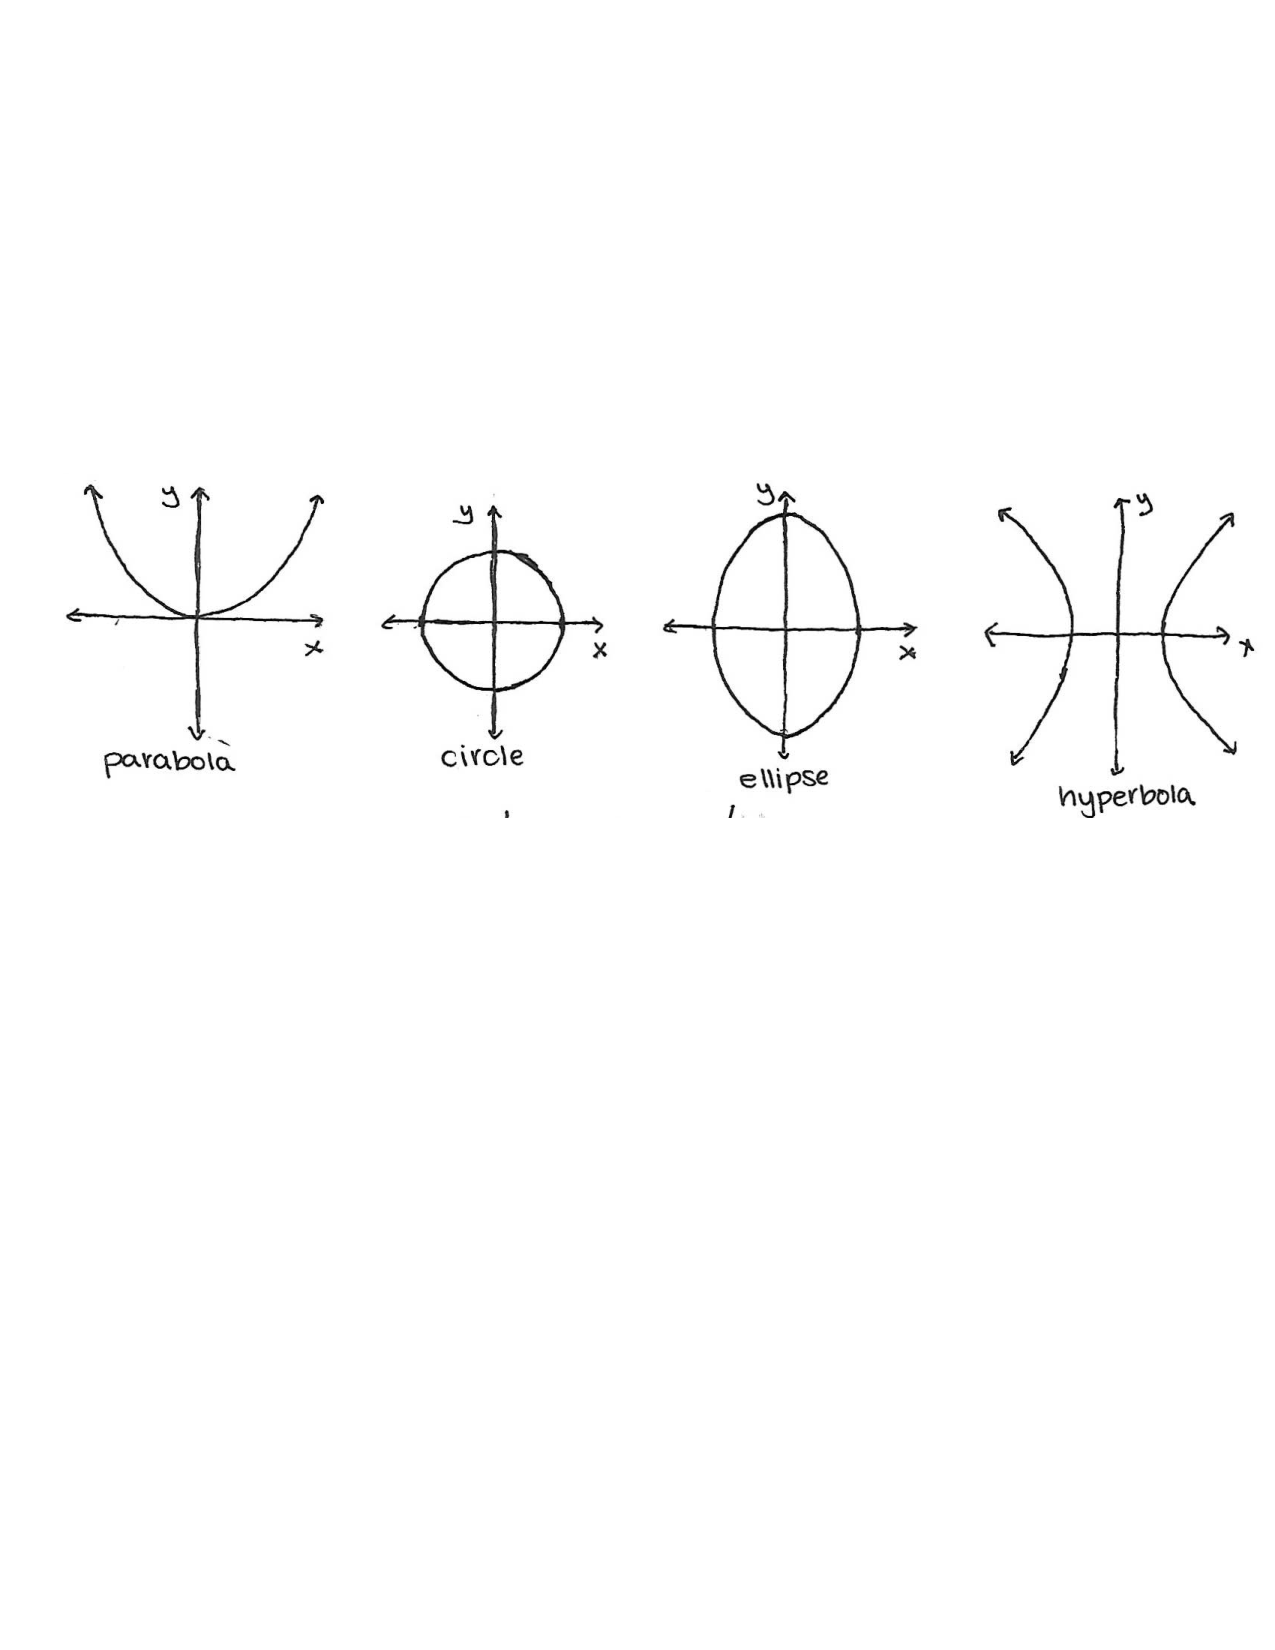
\includegraphics{conics}};
\end{tikzpicture}
\end{image}

Quadric Surfaces are the three dimensional analogue of conic sections. That is, a quadric surface is the set of points in $\mathbb{R}^3$ satisfying some polynomial of degree two in three variables.

\begin{definition}
A \emph{quadric surface} is the set of points $(x,y,z)$ in $\mathbb{R}^3$ satisfying the equation
\[
Ax^2 + Bxy + Cxz + Dy^2 + Eyz + Fz^2 +Gx + Hy + Iz + J = 0,
\]
where $A,B,C,D,E,F,G,H,I,J\in\mathbb{R}$ are constants.
\end{definition}

\section{Simple Forms}

Dealing with quadric surfaces in general can be computationally cumbersome, so we'll focus on quadric surfaces in some simple forms.

\begin{example}
The set of points satisfying
\[
x^2/a^2 + y^2/b^2 + z^2/c^2 = 1,
\]
for some constants $a,b,c\in\mathbb{R}$, is called an \emph{ellipsoid}.

\begin{image}
\begin{tikzpicture}
\node[inner sep=0pt] at (0,0)
    {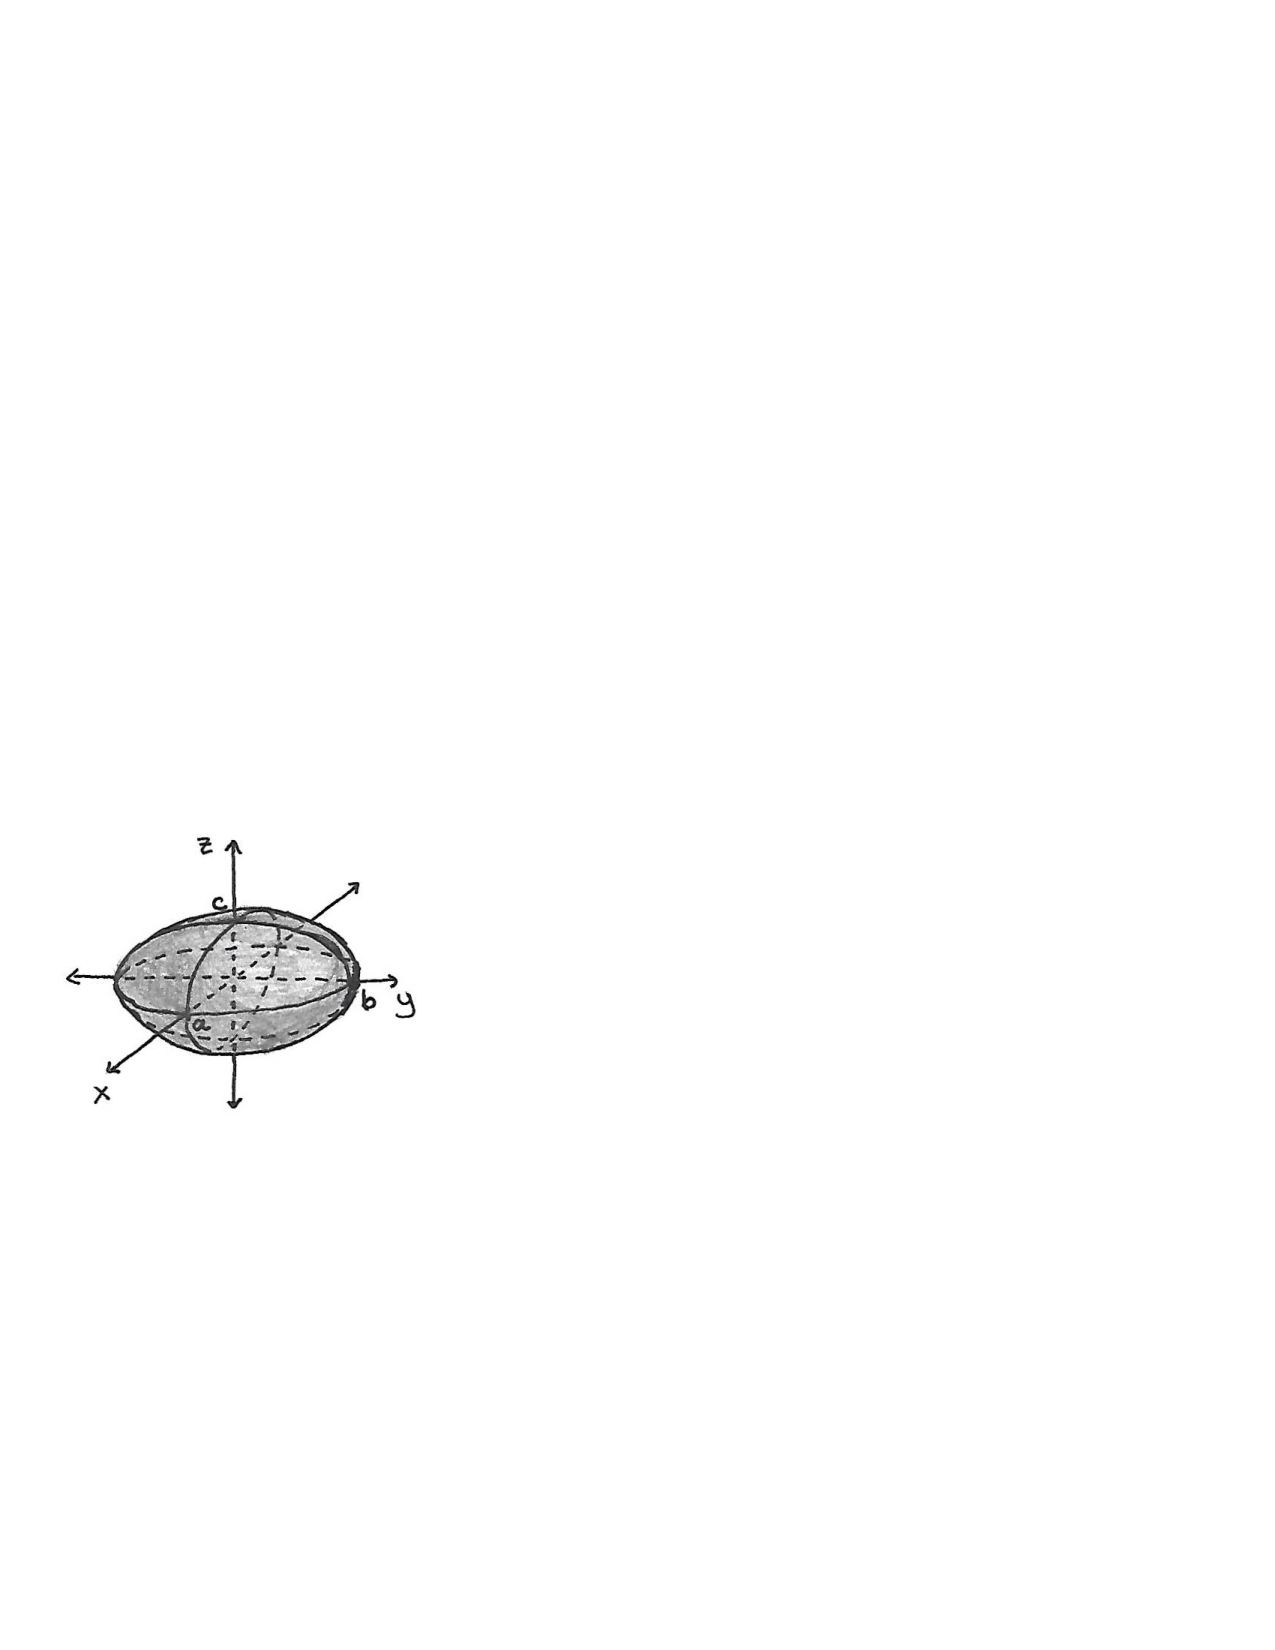
\includegraphics{ellipsoid}};
\end{tikzpicture}
\end{image}

An ellipsoid is kind of like a three dimensional ellipse. In fact, the sections and contour curves of such an an ellipsoid are ellipses.

In the special case that $a=b=c$, this ellipsoid is a sphere of radius $a$.
\end{example}

\begin{example}
The set of points satisfying
\[
z/c = x^2/a^2 + y^2/b^2,
\]
for some constants $a,b,c\in\mathbb{R}$, is called an \emph{elliptic paraboloid}.

\begin{image}
\begin{tikzpicture}
\node[inner sep=0pt] at (0,0)
    {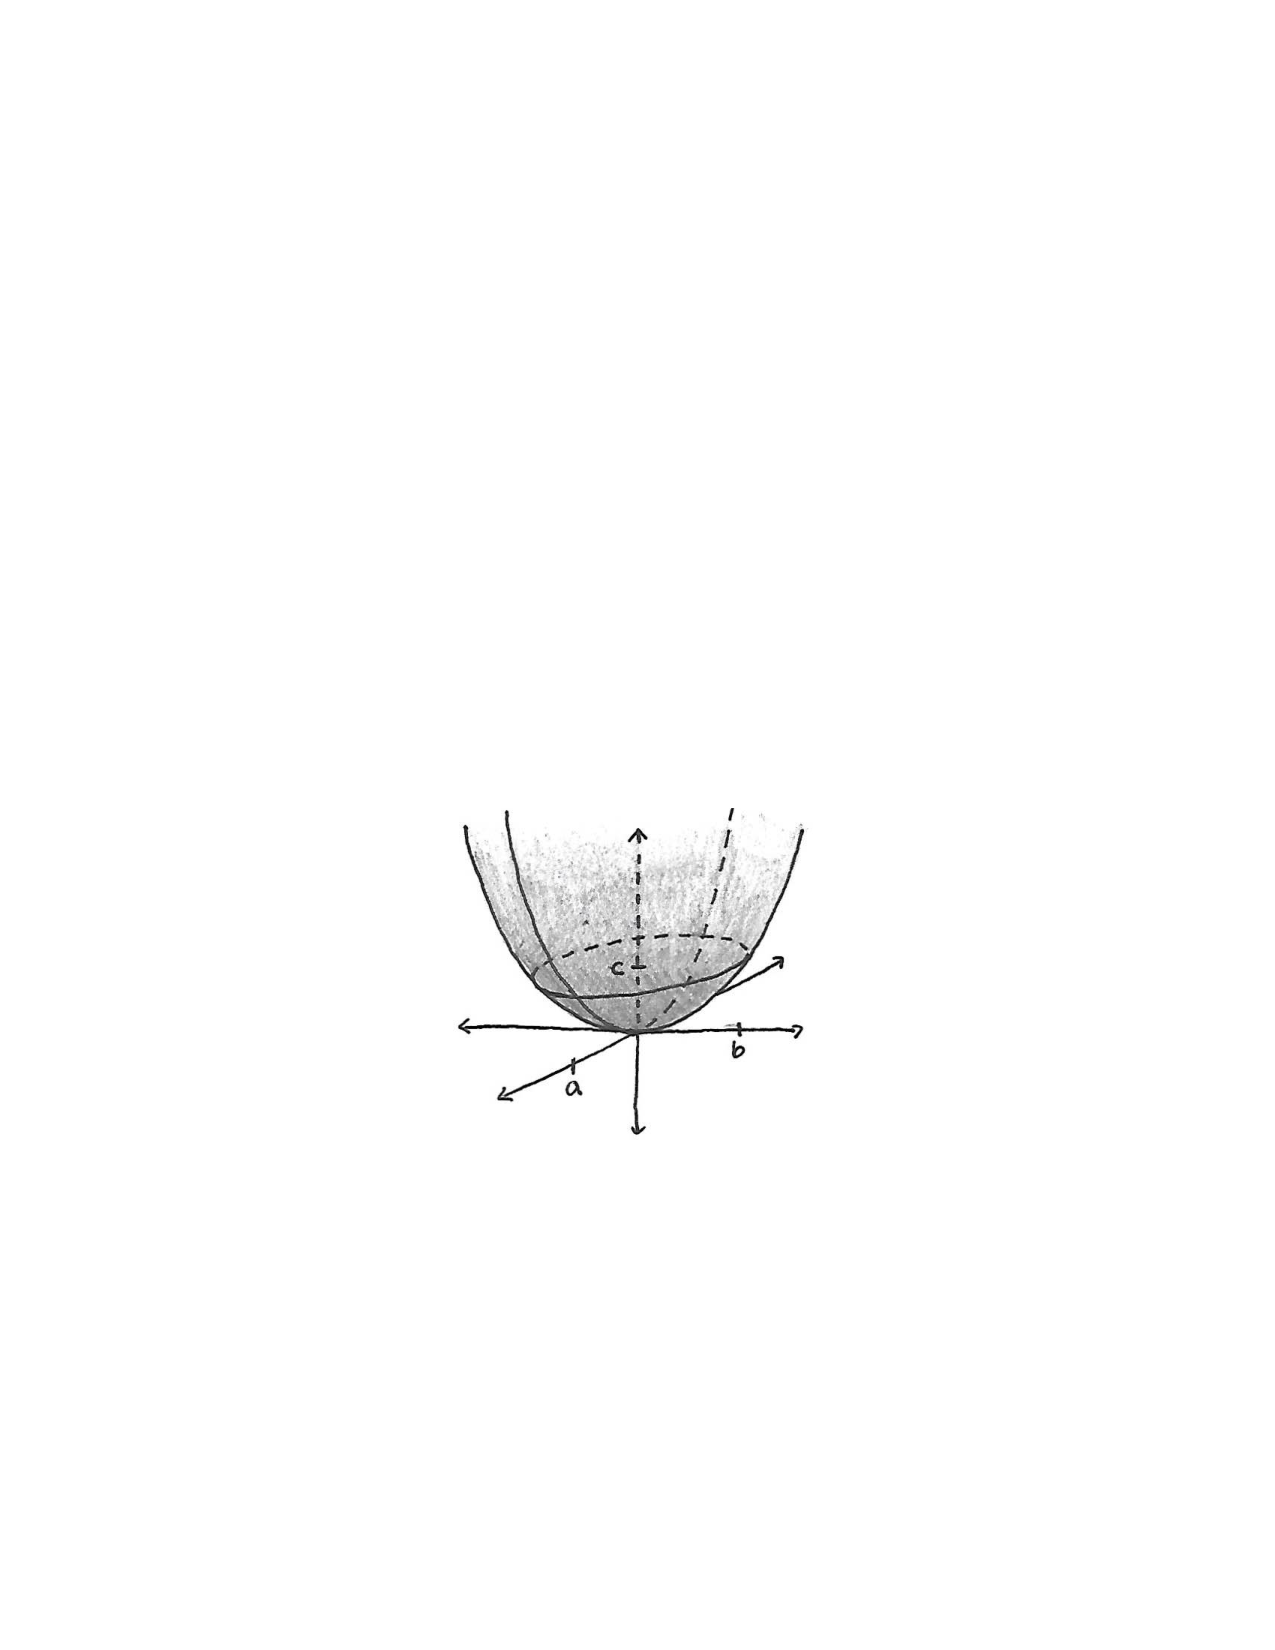
\includegraphics{paraboloid}};
\end{tikzpicture}
\end{image}

The contour curves of such an elliptic paraboloid are ellipses, however the sections are parabolas which all open in the same direction.
\end{example}

\begin{example}
The set of points satisfying
\[
z/c = y^2/b^2 - x^2/a^2,
\]
for some constants $a,b,c\in\mathbb{R}$, is called a \emph{hyperbolic paraboloid}.

\begin{image}
\begin{tikzpicture}
\node[inner sep=0pt] at (0,0)
    {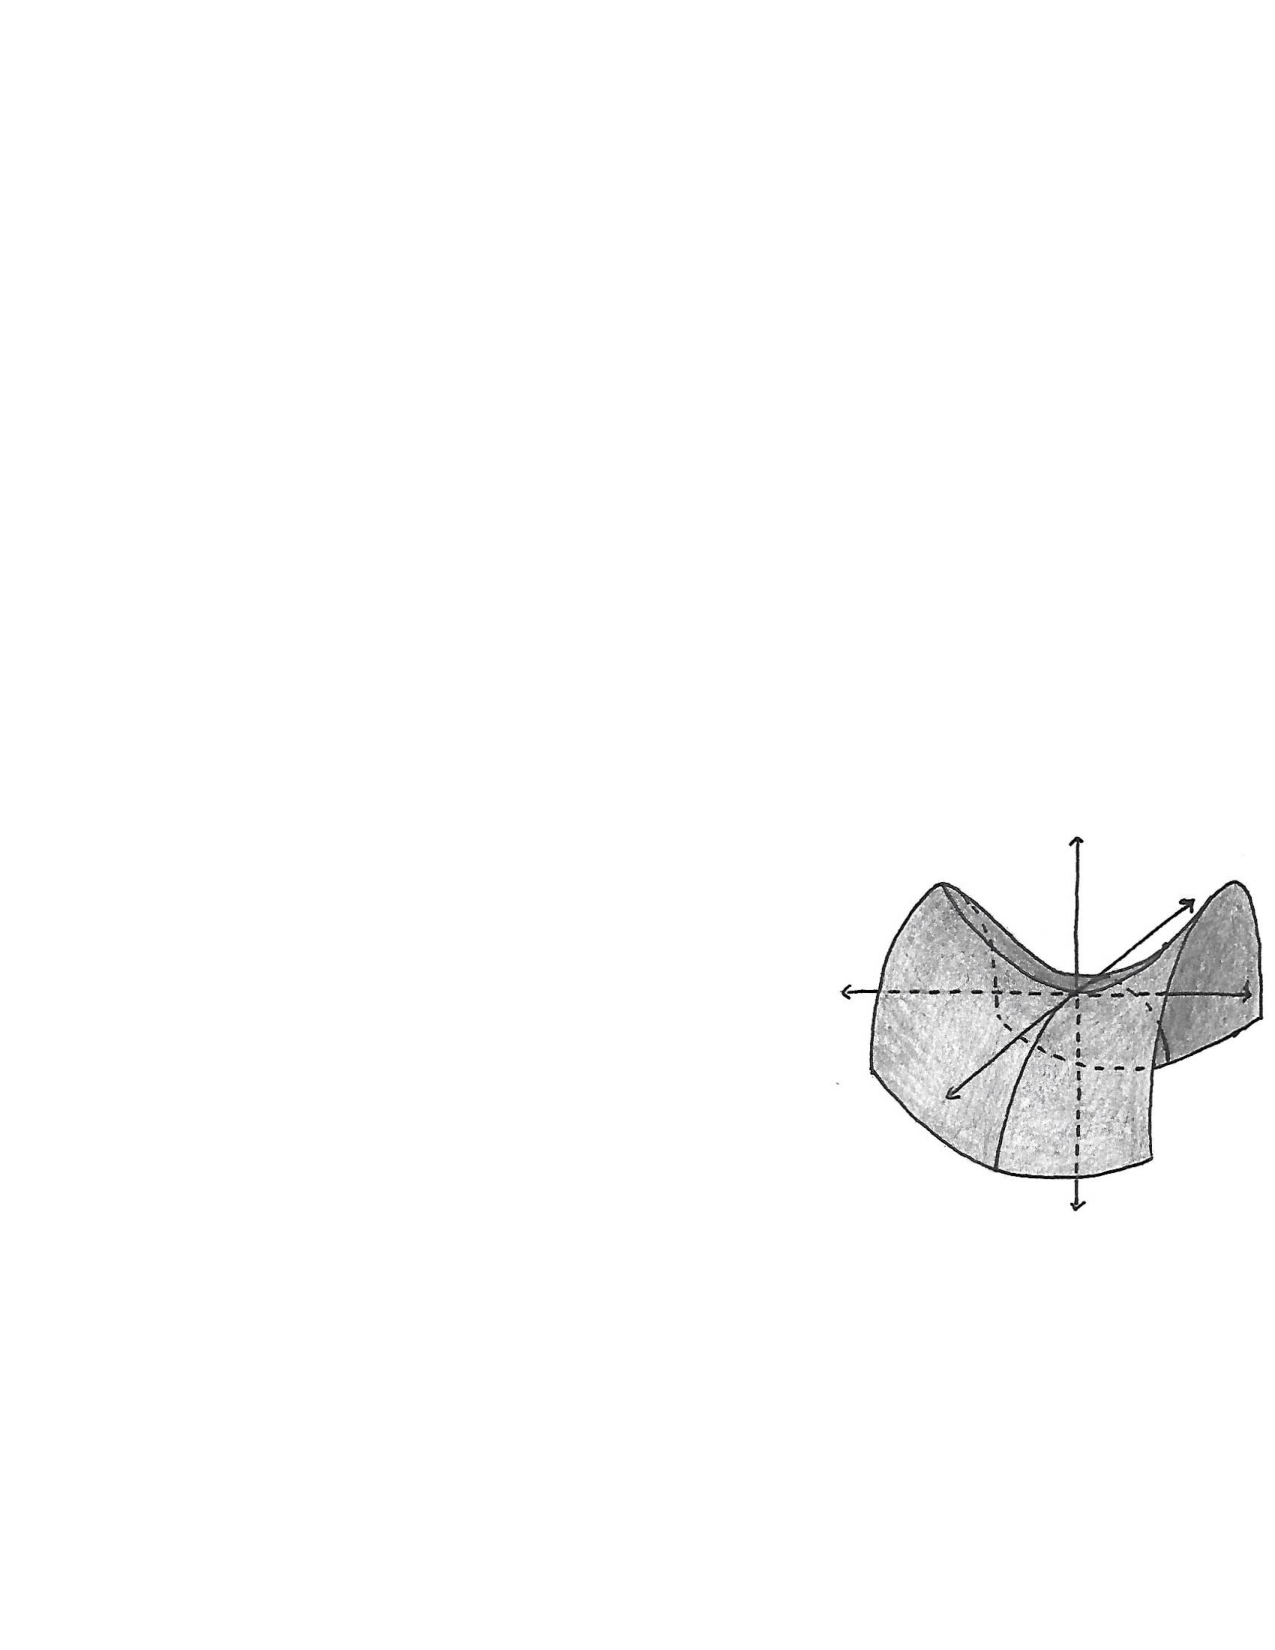
\includegraphics{hyperbolic_paraboloid}};
\end{tikzpicture}
\end{image}

The contour curves of such a hyperbolic paraboloid are hyperbolas, and the sections are parabolas opening in opposite directions for $x$ and $y$ sections. This surface is often described as a ``saddle''.
\end{example}

\begin{example}
The set of points satisfying
\[
z^2/c^2 = x^2/a^2 + y^2/b^2,
\]
for some constants $a,b,c\in\mathbb{R}$, is called an \emph{elliptic cone}.

\begin{image}
\begin{tikzpicture}
\node[inner sep=0pt] at (0,0)
    {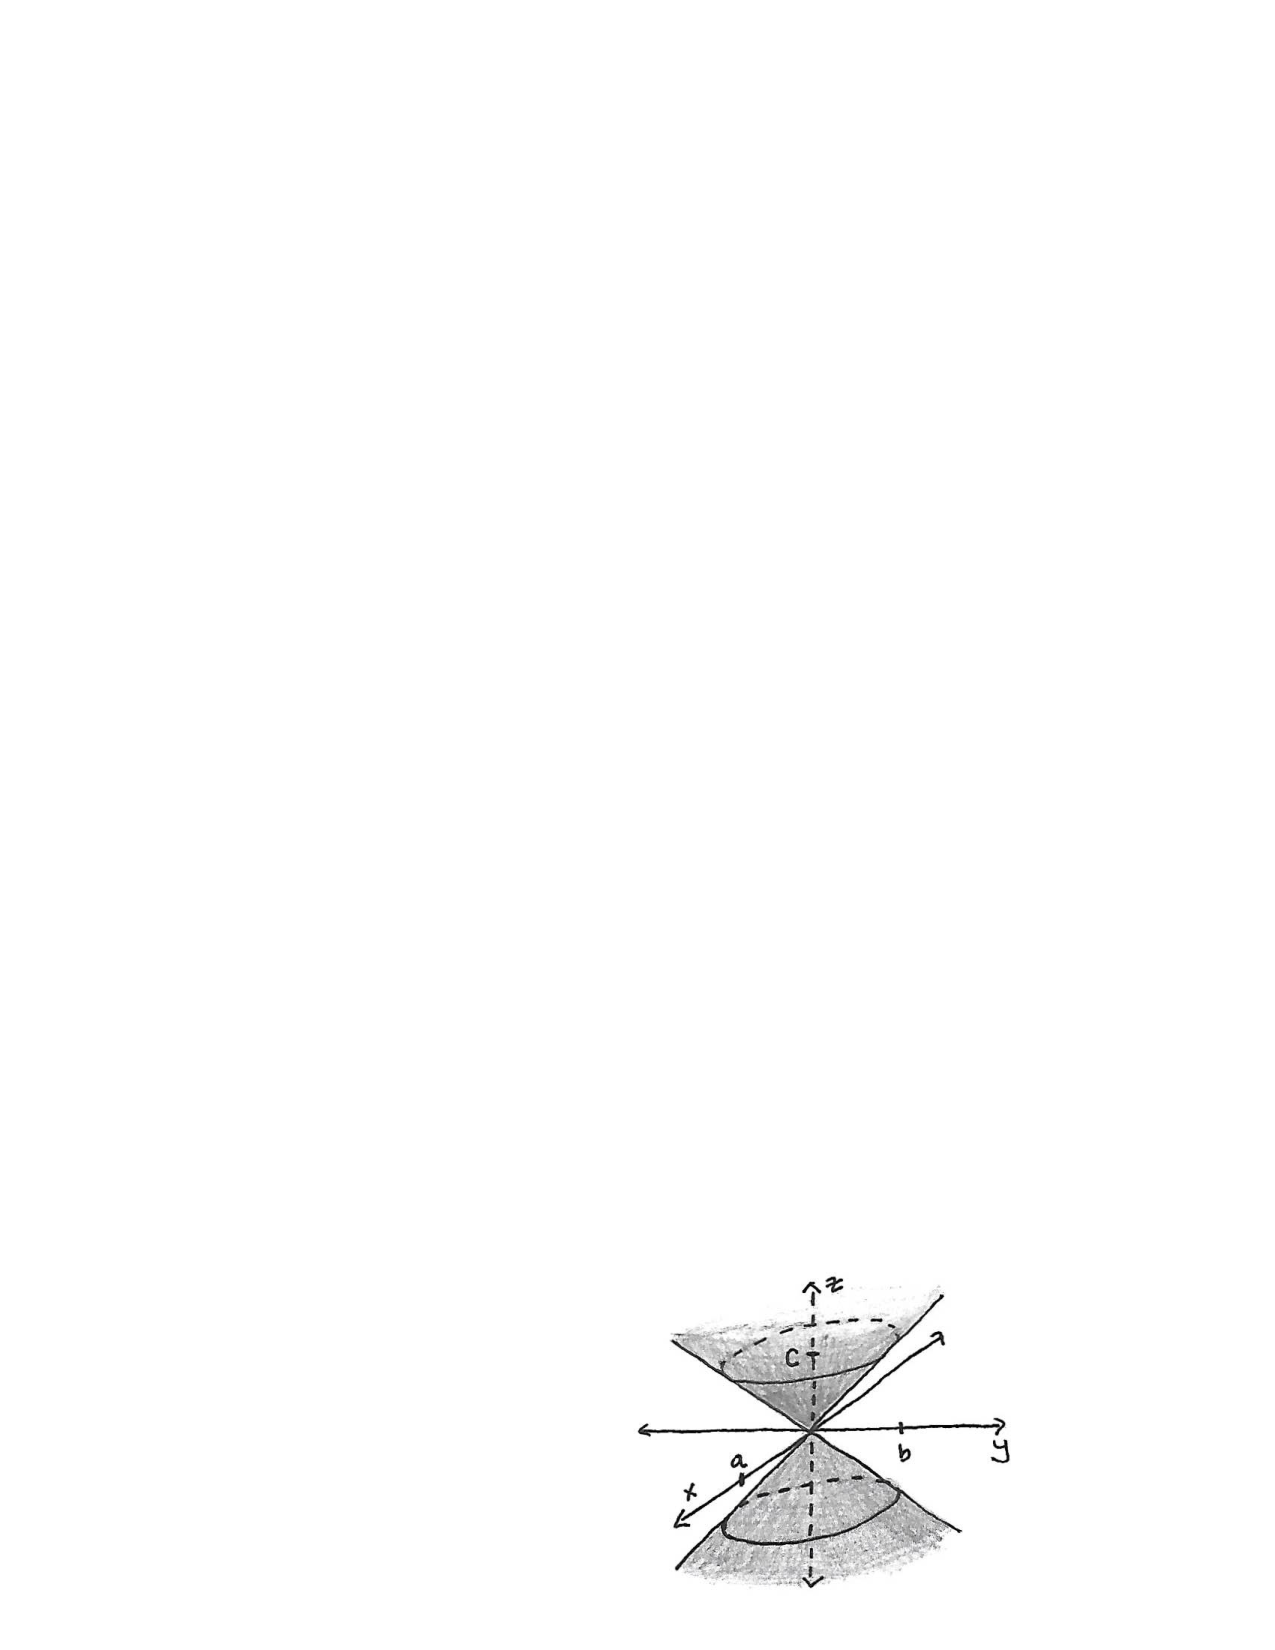
\includegraphics{elliptic_cone}};
\end{tikzpicture}
\end{image}

The contour curves of such an elliptic cone are ellipses, and the sections by $x=0$ and $y=0$ are pairs of intersecting lines.
\end{example}

\begin{example}
The set of points satisfying
\[
x^2/a^2 + y^2/b^2 - z^2/c^2 =1.
\]
for some constants $a,b,c\in\mathbb{R}$, is called a \emph{hyperboloid of one sheet}.

\begin{image}
\begin{tikzpicture}
\node[inner sep=0pt] at (0,0)
    {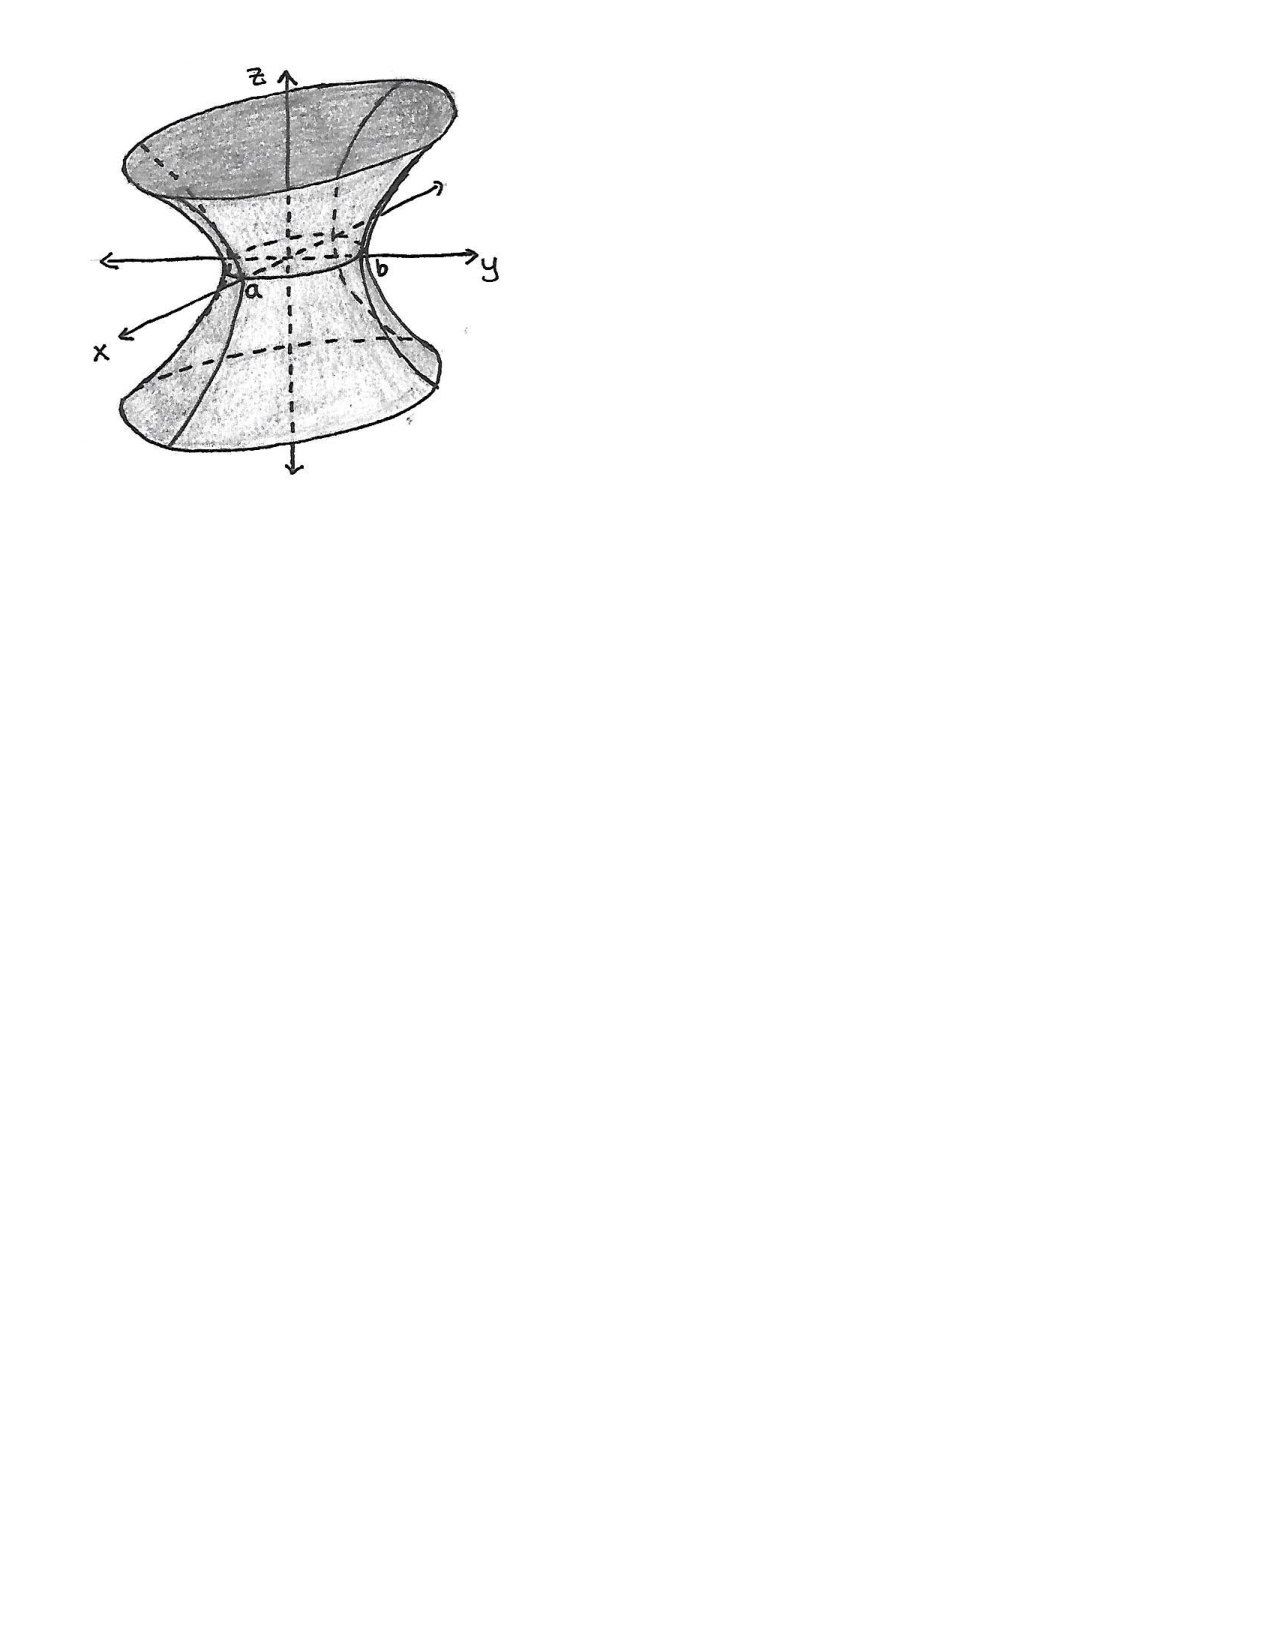
\includegraphics{hyperboloid_one_sheet}};
\end{tikzpicture}
\end{image}

The contour curves of such a hyperboloid are ellipses, and the sections are hyperbolas.
\end{example}

\begin{example}
The set of points satisfying
\[
z^2/c^2 -x^2/a^2 - y^2/b^2 =1.
\]
for some constants $a,b,c\in\mathbb{R}$, is called a \emph{hyperboloid of two sheets}.

\begin{image}
\begin{tikzpicture}
\node[inner sep=0pt] at (0,0)
    {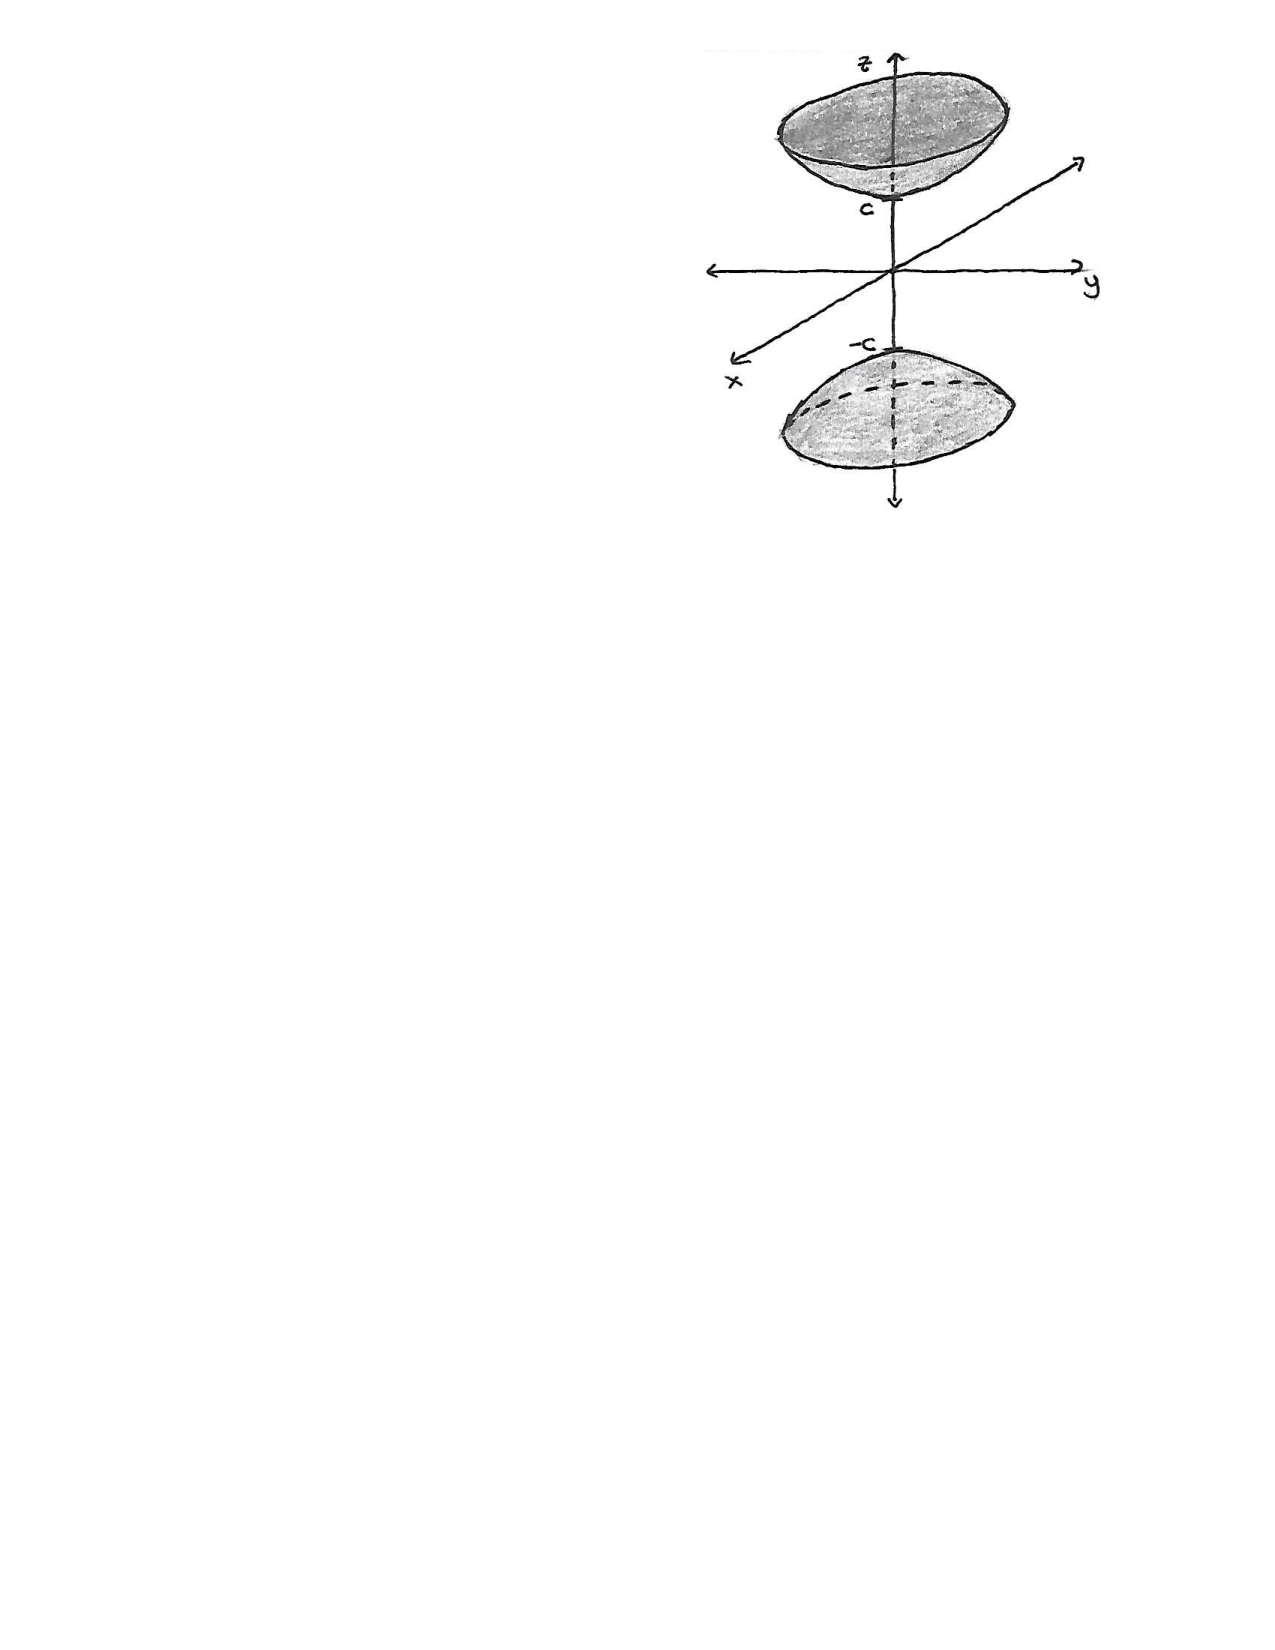
\includegraphics{hyperboloid_two_sheet}};
\end{tikzpicture}
\end{image}

The contour curves of such a hyperboloid are ellipses, and the sections are hyperbolas. We describe this as the hyperboloid ``of two sheets'' since it has two disconnected pieces, as opposed to the hyperboloid of one sheet, which has only one.
\end{example}

APPLET/INTERACTIVE VARYING PARAMETERS

\section{Some Other Forms}

Although we won't really work with quadric surfaces in their most general form, we will consider quadric surfaces that are translations of the forms given above.

For example, the graph of the equation
\[
(x-3)^2 + \frac{(y+2)^2}{3} + \frac{(z-1)^2}{2} = 1
\]
is an ellipsoid centered at $(3,-2,1)$.

PICTURE

However, equations describing quadric surfaces might not always be given to you in easily identifiable forms. In these cases, you might have to do some algebra in order to get the equation into a form where it can be identified as a particular quadric surface. These manipulations will frequently involve completing the square.

We now work through an example of identifying a quadric surface given in a non-standard form.

\begin{example}
Identify the type of quadric surface determined by the equation
\[
-4x^2 + 2y^2 + z^2 + 8x + 4y+4z = 2,
\]
and sketch a graph of this surface.

Our strategy for writing this equation in a recognizable form will be to group terms involving $x$, group terms involving $y$, and group terms involving $z$. We'll then complete the square for each variable.

Grouping terms by variable, we have
\[
(-4x^2+8x) + (2y^2 + 4y) + (z^2 + 4z) = 2.
\]
For each of these grouping, we factor out the leading coefficient, obtaining
\[
\answer{-4}(x^2-2x) + \answer{2}(y^2 + 2y) + (z^2 + 4z) = 2.
\]
We now add or subtract as needed to make the quadratics into squares, getting
\[
-4(x^2-2x + 1) + 2(y^2 + 2y + 1) + (z^2 + 4z + 2) = \answer{4}.
\]
We factor the quadratics to get
\[
-4(\answer{x-1})^2 + 2(\answer{y+1})^2 + (\answer{z+2})^2 = 4.
\]
Finally, we divide by the constant on the right, to get the final form
\[
-(\answer{x-1})^2 + \frac{(\answer{y+1})^2}{2} + \frac{(\answer{z+2})^2}{4} = 1.
\]
We can see that this quadric surface is centered at $\answer{(1,-1,-2)}$, but maybe it still isn't apparent which quadric surface this determines.

Notice that this form is similar to our standard form for a hyperboloid of one sheet, except here it's the $x$-term that's subtracted instead of the $z$-term. This is because this is, in fact, a hyperboloid of one sheet, it just happens to be ``around'' a line parallel to the $x$-axis, rather than a vertical line.

Let's look at a section, in order to help with our sketch. Taking the section $x = 1$, we have an ellipse parallel to the $yz$-plane, centered at $(1,-1,-2)$, with radii $\sqrt{2}$ and $2$.

Combining our observations, we can sketch the graph of this hyperboloid as below.

PICTURE
\end{example}

\section{Conclusion}

In this activity, we introduced and classified quadric surfaces, which form an important family of surfaces.

\end{document}